% ******************************* PhD Thesis Template **************************
% Please have a look at the README.md file for info on how to use the template
%\documentclass[a4paper,11pt,times,numbered,print,index,custommargin]{Classes/PhDThesisPSnPDF}
\documentclass[edeposit,fullpage]{Classes/uiucthesis2009}
\usepackage{booktabs}
\usepackage{multirow}
\usepackage{mathtools}
\usepackage{tabularx}
%\usepackage{geometry}
\usepackage{bm}
\usepackage{setspace}
\usepackage{amsmath}
\usepackage{hyperref}
%A la Bakur's packages
\usepackage{pbox,multirow}
\usepackage[thinlines]{easytable}
\usepackage{lineno}
\usepackage{bigstrut}
\usepackage{enumitem}

%\linenumbers
%\newgeometry{
%    top=3cm,
%   bottom=2.5cm,
%    outer=2.2cm,
%    inner=2.5cm,
%}
\singlespacing
%Newcommands --> define here your alias 
\newcommand{\gvc}{GeV/$c$}
\newcommand{\gvcs}{(GeV/$c$)$^2$}
\newcommand{\gvcw}{GeV/$c^2$}
\newcommand{\mvcw}{MeV/$c^2$}
\newcommand{\mvc}{MeV/$c$}
\newcommand{\diff}{\text{d}}
\newcommand{\siv}{$f_{1,T}^{\, q\perp}(x,\mathbf{k_T})$ }

% ******************************************************************************
% ******************************* Class Options ********************************
% *********************** See README for more details **************************
% ******************************************************************************

% `a4paper'(The University of Cambridge PhD thesis guidelines recommends a page
% size a4 - default option) or `a5paper': A5 Paper size is also allowed as per
% the Cambridge University Engineering Deparment guidelines for PhD thesis
%
% `11pt' or `12pt'(default): Font Size 10pt is NOT recommended by the University
% guidelines
%
% `oneside' or `twoside'(default): Printing double side (twoside) or single
% side.
%
% `print': Use `print' for print version with appropriate margins and page
% layout. Leaving the options field blank will activate Online version.
%
% `index': For index at the end of the thesis
%
% `draft': For draft mode without loading any images (same as draft in book)
%
% `draftmode': Special draft mode with line numbers, images, and water mark with
% timestamp and custom text. Position of the text can also be modified.
%
% `abstract': To generate only the title page and abstract page with
% dissertation title and name, to submit to the Student Registry
%
% `chapter`: This option enables only the specified chapter and it's references
%  Useful for review and corrections.
%
% ************************* Custom Page Margins ********************************
%
% `custommargin`: Use `custommargin' in options to activate custom page margins,
% which can be defined in the preamble.tex. Custom margin will override
% print/online margin setup.
%
% *********************** Choosing the Fonts in Class Options ******************
%
% `times' : Times font with math support. (The Cambridge University guidelines
% recommend using times)
%
% `fourier': Utopia Font with Fourier Math font (Font has to be installed)
%            It's a free font.
%
% `customfont': Use `customfont' option in the document class and load the
% package in the preamble.tex
%
% default or leave empty: `Latin Modern' font will be loaded.
%
% ********************** Choosing the Bibliography style ***********************
%
% `authoryear': For author-year citation eg., Krishna (2013)
%
% `numbered': (Default Option) For numbered and sorted citation e.g., [1,5,2]
%
% `custombib': Define your own bibliography style in the `preamble.tex' file.
%              `\RequirePackage[square, sort, numbers, authoryear]{natbib}'.
%              This can be also used to load biblatex instead of natbib
%              (See Preamble)
%
% **************************** Choosing the Page Style *************************
%
% `default (leave empty)': For Page Numbers in Header (Left Even, Right Odd) and
% Chapter Name in Header (Right Even) and Section Name (Left Odd). Blank Footer.
%
% `PageStyleI': Chapter Name next & Page Number on Even Side (Left Even).
% Section Name & Page Number in Header on Odd Side (Right Odd). Footer is empty.
%
% `PageStyleII': Chapter Name on Even Side (Left Even) in Header. Section Number
% and Section Name in Header on Odd Side (Right Odd). Page numbering in footer


% ********************************** Preamble **********************************
% Preamble: Contains packages and user-defined commands and settings
% ******************************************************************************
% ****************************** Custom Margin *********************************

% Add `custommargin' in the document class options to use this section
% Set {innerside margin / outerside margin / topmargin / bottom margin}  and
% other page dimensions
%%\ifsetCustomMargin
%%  \RequirePackage[left=25mm,right=22mm,top=30mm,bottom=25mm]{geometry}
%%  \setFancyHdr % To apply fancy header after geometry package is loaded
%%\fi

% *****************************************************************************
% ******************* Fonts (like different typewriter fonts etc.)*************

% Add `customfont' in the document class option to use this section

%%\ifsetCustomFont
%%  % Set your custom font here and use `customfont' in options. Leave empty to
%%  % load computer modern font (default LaTeX font).
%%  \RequirePackage{helvet}
%%\fi

% *****************************************************************************
% **************************** Custom Packages ********************************

% ************************* Algorithms and Pseudocode **************************

%\usepackage{algpseudocode}


% ********************Captions and Hyperreferencing / URL **********************

% Captions: This makes captions of figures use a boldfaced small font.
%\RequirePackage[small,bf]{caption}

\RequirePackage[labelsep=space,tableposition=top]{caption}
\renewcommand{\figurename}{Figs} %to support older versions of captions.sty


% *************************** Graphics and figures *****************************

%\usepackage{rotating}
%\usepackage{wrapfig}

% Uncomment the following two lines to force Latex to place the figure.
% Use [H] when including graphics. Note 'H' instead of 'h'
%\usepackage{float}
%\restylefloat{figure}

% Subcaption package is also available in the sty folder you can use that by
% uncommenting the following line
% This is for people stuck with older versions of texlive
%\usepackage{sty/caption/subcaption}
\usepackage{subcaption}

% ********************************** Tables ************************************
\usepackage{booktabs} % For professional looking tables
\usepackage{multirow}

%\usepackage{multicol}
%\usepackage{longtable}
%\usepackage{tabularx}


% ***************************** Math and SI Units ******************************

\usepackage{amsfonts}
\usepackage{amsmath}
\usepackage{amssymb}
\usepackage{siunitx} % use this package module for SI units


% ******************************* Line Spacing *********************************

% Choose linespacing as appropriate. Default is one-half line spacing as per the
% University guidelines

% \doublespacing
% \onehalfspacing
% \singlespacing


% ************************ Formatting / Footnote *******************************

% Don't break enumeration (etc.) across pages in an ugly manner (default 10000)
%\clubpenalty=500
%\widowpenalty=500

%\usepackage[perpage]{footmisc} %Range of footnote options


% *****************************************************************************
% *************************** Bibliography  and References ********************

%\usepackage{cleveref} %Referencing without need to explicitly state fig /table

% Add `custombib' in the document class option to use this section
%%\ifuseCustomBib
%%   \RequirePackage[square, sort, numbers, authoryear]{natbib} % CustomBib
%%
%%% If you would like to use biblatex for your reference management, as opposed to the default `natbibpackage` pass the option `custombib` in the document class. Comment out the previous line to make sure you don't load the natbib package. Uncomment the following lines and specify the location of references.bib file
%%
%%%\RequirePackage[backend=biber, style=numeric-comp, citestyle=numeric, sorting=nty, natbib=true]{biblatex}
%%%\bibliography{References/references} %Location of references.bib only for biblatex
%%
%%\fi

% changes the default name `Bibliography` -> `References'
\renewcommand{\bibname}{References}


% *****************************************************************************
% *************** Changing the Visual Style of Chapter Headings ***************
% This section on visual style is from https://github.com/cambridge/thesis

% Uncomment the section below. Requires titlesec package.

%\RequirePackage{titlesec}
%\newcommand{\PreContentTitleFormat}{\titleformat{\chapter}[display]{\scshape\Large}
%{\Large\filleft{\chaptertitlename} \Huge\thechapter}
%{1ex}{}
%[\vspace{1ex}\titlerule]}
%\newcommand{\ContentTitleFormat}{\titleformat{\chapter}[display]{\scshape\huge}
%{\Large\filleft{\chaptertitlename} \Huge\thechapter}{1ex}
%{\titlerule\vspace{1ex}\filright}
%[\vspace{1ex}\titlerule]}
%\newcommand{\PostContentTitleFormat}{\PreContentTitleFormat}
%\PreContentTitleFormat


% ******************************************************************************
% ************************* User Defined Commands ******************************
% ******************************************************************************

% *********** To change the name of Table of Contents / LOF and LOT ************

%\renewcommand{\contentsname}{My Table of Contents}
%\renewcommand{\listfigurename}{My List of Figures}
%\renewcommand{\listtablename}{My List of Tables}


% ********************** TOC depth and numbering depth *************************

\setcounter{secnumdepth}{2}
\setcounter{tocdepth}{2}


% ******************************* Nomenclature *********************************

% To change the name of the Nomenclature section, uncomment the following line

%\renewcommand{\nomname}{Symbols}


% ********************************* Appendix ***********************************

% The default value of both \appendixtocname and \appendixpagename is `Appendices'. These names can all be changed via:

%\renewcommand{\appendixtocname}{List of appendices}
%\renewcommand{\appendixname}{Appndx}

% ******************************** Draft Mode **********************************

% Uncomment to disable figures in `draftmode'
%\setkeys{Gin}{draft=true}  % set draft to false to enable figures in `draft'

% These options are active only during the draft mode
% Default text is "Draft"
%\SetDraftText{DRAFT}

% Default Watermark location is top. Location (top/bottom)
%\SetDraftWMPosition{bottom}

% Draft Version - default is v1.0
%\SetDraftVersion{v1.1}

% Draft Text grayscale value (should be between 0-black and 1-white)
% Default value is 0.75
%\SetDraftGrayScale{0.8}


%% Todo notes functionality
%% Uncomment the following lines to have todonotes.

%\ifsetDraft
%	\usepackage[colorinlistoftodos]{todonotes}
%	\newcommand{\mynote}[1]{\todo[author=kks32,size=\small,inline,color=green!40]{#1}}
%\else
%	\newcommand{\mynote}[1]{}
%	\newcommand{\listoftodos}{}
%\fi

% Example todo: \mynote{Hey! I have a note}




% ************************ Thesis Information & Meta-data **********************
% Thesis title and author information, refernce file for biblatex
%% ************************ Thesis Information & Meta-data **********************
%% The title of the thesis
\title{Universit\`a degli Studi di Torino \\
{\bf Scuola di Dottorato in Scienza ed Alta Tecnologia} \\}
%\texorpdfstring is used for PDF metadata. Usage:
%\texorpdfstring{LaTeX_Version}{PDF Version (non-latex)} eg.,
%\texorpdfstring{$sigma$}{sigma}

%% Subtitle (Optional)
\subtitle{Using the CUED template}

%% The full name of the author
\author{Krishna Kumar}

%% Department (eg. Department of Engineering, Maths, Physics)
\dept{Department of Engineering}

%% University and Crest
\university{Universit\`a degli Studi di Torino \\
{\bf Scuola di Dottorato in Scienza ed Alta Tecnologia} \\}
\crest{\includegraphics[width=0.25\textwidth]{University_Crest}}

%% You can redefine the submission text:
% Default as per the University guidelines:
% ``This dissertation is submitted for the degree of''
%\renewcommand{\submissiontext}{change the default text here if needed}

%% Full title of the Degree
\degree{Doctor of Philosophy}

%% College affiliation (optional)
\college{King's College}

%% Submission date
% Default is set as {\monthname[\the\month]\space\the\year}
%\degreedate{September 2014} 

%% Meta information
\subject{LaTeX} \keywords{{LaTeX} {PhD Thesis} {Engineering} {University of
Cambridge}}




% ***************************** Abstract Separate ******************************
% To printout only the titlepage and the abstract with the PhD title and the
% author name for submission to the Student Registry, use the `abstract' option in
% the document class.

%\ifdefineAbstract
%\pagestyle{empty}
 %\includeonly{Declaration/declaration, Abstract/abstract}
%\fi

% ***************************** Chapter Mode ***********************************
% The chapter mode allows user to only print particular chapters with references
% Title, Contents, Frontmatter are disabled by default
% Useful option to review a particular chapter or to send it to supervisior.
% To use choose `chapter' option in the document class

%\ifdefineChapter
 %\includeonly{Chapter3/chapter3}
%\fi

% ******************************** Front Matter ********************************
\begin{document}
  
%\documentclass[a4paper,12pt]{article}

%%%%%%%%%%%%%%%%%%%%%%%%%%%%%%%%%%%%%%%%%%%%%%%%%%%%%%%%%%
%\begin{document}

\thispagestyle{empty}
\begin{center}
\begin{large}
University of Illinois at Urbana-Champaign \\
{\bf Degree of Doctor of Physics} \\
%{\bf XXX Ciclo}
\end{large}
\end{center}
\hrulefill

\vspace{1cm}
\begin{center}

\includegraphics[width=6cm]{Figs/illini.png}
\end{center}
\vspace{2cm}
\begin{center}
\Large{\bf Drell-Yan at COMPASS rocks it!}
\end{center}
\vspace{2cm}
\large{\bf Candidate: Robert Shannon Heitz} \vspace{0.5cm}\newline
\large{\bf Supervisor: Prof. Matthias Grosse-Perdekamp} \\
\large{\bf Supervisor: Prof. Caroline Riedl} \vspace{0.5cm}\newline
%\end{document}
%%%%%%%%%%%%%%%%%%%%%%%%%%%%%%%%%%%%%%%%%%%%%%%%%%%%%%%%%%
%\newpage
%\pagenumbering{arabic}
%\begin{center}
%\begin{large}
%Universit\`a degli Studi di Torino \\
%{\bf Scuola~di~Dottorato~in~Scienza~ed~Alta~Tecnologia}
%\end{large}
%\end{center}
%\hrulefill
%\begin{center}
%\begin{large}
%{\bf Tesi di Dottorato di Ricerca in Scienza ed Alta Tecnologia} \\
%{\bf Indirizzo di Fisica ed Astrofisica}
%\end{large}
%\end{center}

%%\vspace{2cm}
%\Large{\bf Titolo titolo titolo titolo titolo titolo titolo}

%\vspace{8cm}
%\large{\bf Nome e cognome del dottorando}

%\vspace{1cm}
%\large{\bf Tutor: Nome e cognome del relatore}

%\end{document} 


%\frontmatter
%\begin{titlepage}
  %\maketitle
%\end{titlepage}

\renewcommand{\thepage}{\roman{page}}
% ******************************* Thesis Dedidcation ********************************

\begin{dedication} 
To whom it may concern 
\end{dedication}


%% ******************************* Thesis Declaration ********************************

\begin{declaration}

I hereby declare that except where specific reference is made to the work of others, the contents of this dissertation are original and have not been submitted in whole or in part for consideration for any other degree or qualification in this, or any other University. This dissertation is the result of my own work and includes nothing which is the outcome of work done in collaboration, except where specifically indicated in the text. This dissertation contains less than 65,000 words including appendices, bibliography, footnotes, tables and equations and has less than 150 figures.

% Author and date will be inserted automatically from thesis.tex \author \degreedate

\end{declaration}


% ************************** Thesis Abstract *****************************
% Use `abstract' as an option in the document class to print only the titlepage and the abstract.
\begin{abstract}
Dear Barbara Badelek, hereafter my abstract 

\end{abstract}

%%% ************************** Thesis Acknowledgements *****************************

\begin{acknowledgements}      
Thanks everyone for joining. It was nice, but I would not repeat it! \end{acknowledgements}


% *********************** Adding TOC and List of Figures ***********************
\tableofcontents

% \printnomencl[space] space can be set as 2em between symbol and description
%\printnomencl[3em]
%%\printnomencl
\clearpage
\renewcommand{\thepage}{\arabic{page}}
% ******************************** Main Matter *********************************
\mainmatter
\addcontentsline{toc}{chapter}{Introduction}  

%Chapter 1 
\chapter{Measurement of the Left Right Asymmetry in the Drell-Yan Process} 
\label{Chap:setup}
\ifpdf
\graphicspath{{Chapters/OneCh/Figs/Raster/}{Chapters/OneCh/Figs/PDF/}{Chapters/OneCh/Figs/}}
\else \graphicspath{{Chapters/OneCh/Figs/Vector/}{Chapters/OneCh/Figs/}} \fi

Introduction about L/R asym.  In this Chapter....  Define AN

\section{Data Sample}
The data sample comes from the 2015 COMPASS Drell-Yan measurement where a 190
GeV/c $\pi^-$ beam impinged on a transversely polarized NH$_3$ target.  The
stable data comes from July 8, through November 12 and is split into 9 periods
lasting approximated 2 weeks each where each period consist of two sub-periods.
To reduce systematics, the NH$_3$ was split into two oppositely polarized cells
separated by 20 cm and the polarization of both cells was flipped between
sub-periods.  A summary of the data taking from each period is shown in table
~\ref{tab::datataking}.

\begin{table}[h!]
  \centering
    \begin{tabular}{ |c|c|c|c|c|c| }
      \hline
      Period&  Sub-period&  Polarization&  First-Last run&  Begin date&  End date \\
      \hline
      
      \multirow{2}{2em}{W07}&  one&  $\downarrow \uparrow$&  259363 - 259677&  July 9&  July 15 \\
      & two&  $\uparrow \downarrow$&  259744 - 260016&  July 16&  July 22 \\
      \hline

      \multirow{2}{2em}{W08}&  one&  $\uparrow \downarrow$&  260074 - 260264&  July 23&  July 29 \\
      & two&  $\downarrow \uparrow$&  260317 - 260565&  July 29&  August 5 \\
      \hline

      \multirow{2}{2em}{W09}&  one&  $\downarrow \uparrow$&  260627 - 260852&  August 5&  August 12 \\
      & two&  $\uparrow \downarrow$&  260895 - 261496&  August 12&  August 26 \\
      \hline

      \multirow{2}{2em}{W10}&  one&  $\uparrow \downarrow$&  261515 - 261761&  August 26&  September 1 \\
      & two&  $\downarrow \uparrow$&  261970 - 262221&  September 4&  September 9 \\
      \hline

      \multirow{2}{2em}{W11}&  one&  $\downarrow \uparrow$&  262370 - 262772&  September 11&  September 22 \\
      & two&  $\uparrow \downarrow$&  262831 - 263090&  September 23&  September 30 \\
      \hline

      \multirow{2}{2em}{W12}&  one&  $\uparrow \downarrow$&  263143 - 263347&  September 30&  October 7 \\
      & two&  $\downarrow \uparrow$&  263386 - 263603&  October 8&  October 14 \\
      \hline

      \multirow{2}{2em}{W13}&  one&  $\downarrow \uparrow$&  263655 - 263853&  October 15&  October 21 \\
      & two&  $\uparrow \downarrow$&  263926 - 264134&  October 22&  October 28 \\
      \hline

      \multirow{2}{2em}{W14}&  one&  $\uparrow \downarrow$&  264170 - 264330&  October 28&  November 2 \\
      & two&  $\downarrow \uparrow$&  264429 - 264562&  November 4&  November 8 \\
      \hline

      \multirow{2}{2em}{W15}&  one&  $\downarrow \uparrow$&  264619 - 264672&  November 9&  November 11 \\
      & two&  $\uparrow \downarrow$&  264736 - 264857&  November 12&  November 16 \\
      \hline
      
    \end{tabular}
    \caption{COMPASS 2015 data taking periods}
    \label{tab::datataking}
  \end{table}


\subsection{Event Selection}
The cuts in the event selection were chosen to ensure the final state consisted
of dimuons resulting from a pion collision in the transversely polarized target.
The event selection was initial filtered from miniDSTs to $\mu$DSTs using the
criteria of at least two muons in the final state.  The following event
selection is performed on these $\mu$DSTs where the events used come from the
slot1 production.  A summary of the number of events remaining after each cut is
shown in figure~\ref{fig::EventTable}.
\begin{itemize}
\item Two oppositely charged particles from a common best primary vertex.  The
  criteria for a primary vertex is any vertex with an associated beam particle.
  In case of multiple common vertices the best primary vertex was determined by
  CORAL tagging the vertex as best primary (PHAST method
  PaVertex::IsBestPrimary()).  If CORAL did not tag any of the common vertices
  as the best primary the vertex with the smallest spatial chi$^2$ value was
  used as the best primary vertex.
\item A dimuon trigger fired.  A dimuon trigger firing means there are at least
  two particles in coincidence in this event. The dimuon triggers used were a
  coincidence between two particles in the large angle spectrometer, LAS-LAS
  trigger, or a particle in the large angle spectrometer and a particle in the
  Outer hodoscope in the small angle spectrometer, LAS-Outer trigger.  The
  LAS-Middle trigger was used a veto on beam decay muons.  This is because the
  LAS-Middle trigger was found to have many events resulting from a beam pion
  decaying to a muon.
\item Both particles are muons.  A muon was defined as having crossed 30
  radiation lengths of material between the particles first and last measured
  points.  This criteria has been previously determined to be effective at
  distinguishing between muons and hadrons.  In the final production no
  detectors were used from upstream of the hadron absorber so the absorber is
  not included in the determination of material crossed.
\item The first measured point for both particles is before 300 cm and the last
  measured point is after 1500 cm.  This cut ensures both particles have
  positions upstream of the first spectrometer magnet and downstream of the
  first muon filter.
\item The timing of both muons is defined.  This checks that the time relative
  to the trigger time is determined for both muons so further timing cuts can be
  performed.
\item Both muons are in time within 5 nanoseconds.  This cut helps rejected
  uncorrelated muons.
\item The muon tracks reduced chi$^2$ are individually less than 10.  This cut
  ensure track quality.
\item A validation that each muon crossed the trigger it was associated as
  having triggered.  This trigger validation cut was performed by extrapolating
  (PHAST Method PaTrack::Extrapolate()) each muon track back to the hodoscopes
  it fired and determining if the muon crossed the geometric acceptance of both
  hodoscopes.
\item The event does not occur in the bad spill or run list.
\item The Drell-Yan kinematics are physical.  That is the beam and target
  x-Bjorken are between 0 and 1 and x-Feynman is between -1 and 1.
\item The transverse momentum of the virtual photon is between 0.4 and 5.0
  GeV/c.  The lower limit ensures azimuthal angular resolution is sufficient and
  the upper cut is minimal and ensure physical kinematics.
\item The vertex originated within the z-positions of the transversely polarized
  targets defined by the target group (-294.5$<$ Z$_{\mathrm{vertex}}$ $<$-239.3
  or -219.5$<$ Z$_{\mathrm{vertex}}$ $<$-164.3 cm).
\item The vertex is within the radius of the target defined as 1.9 cm.
\end{itemize}

\begin{figure}
  \begin{center}
    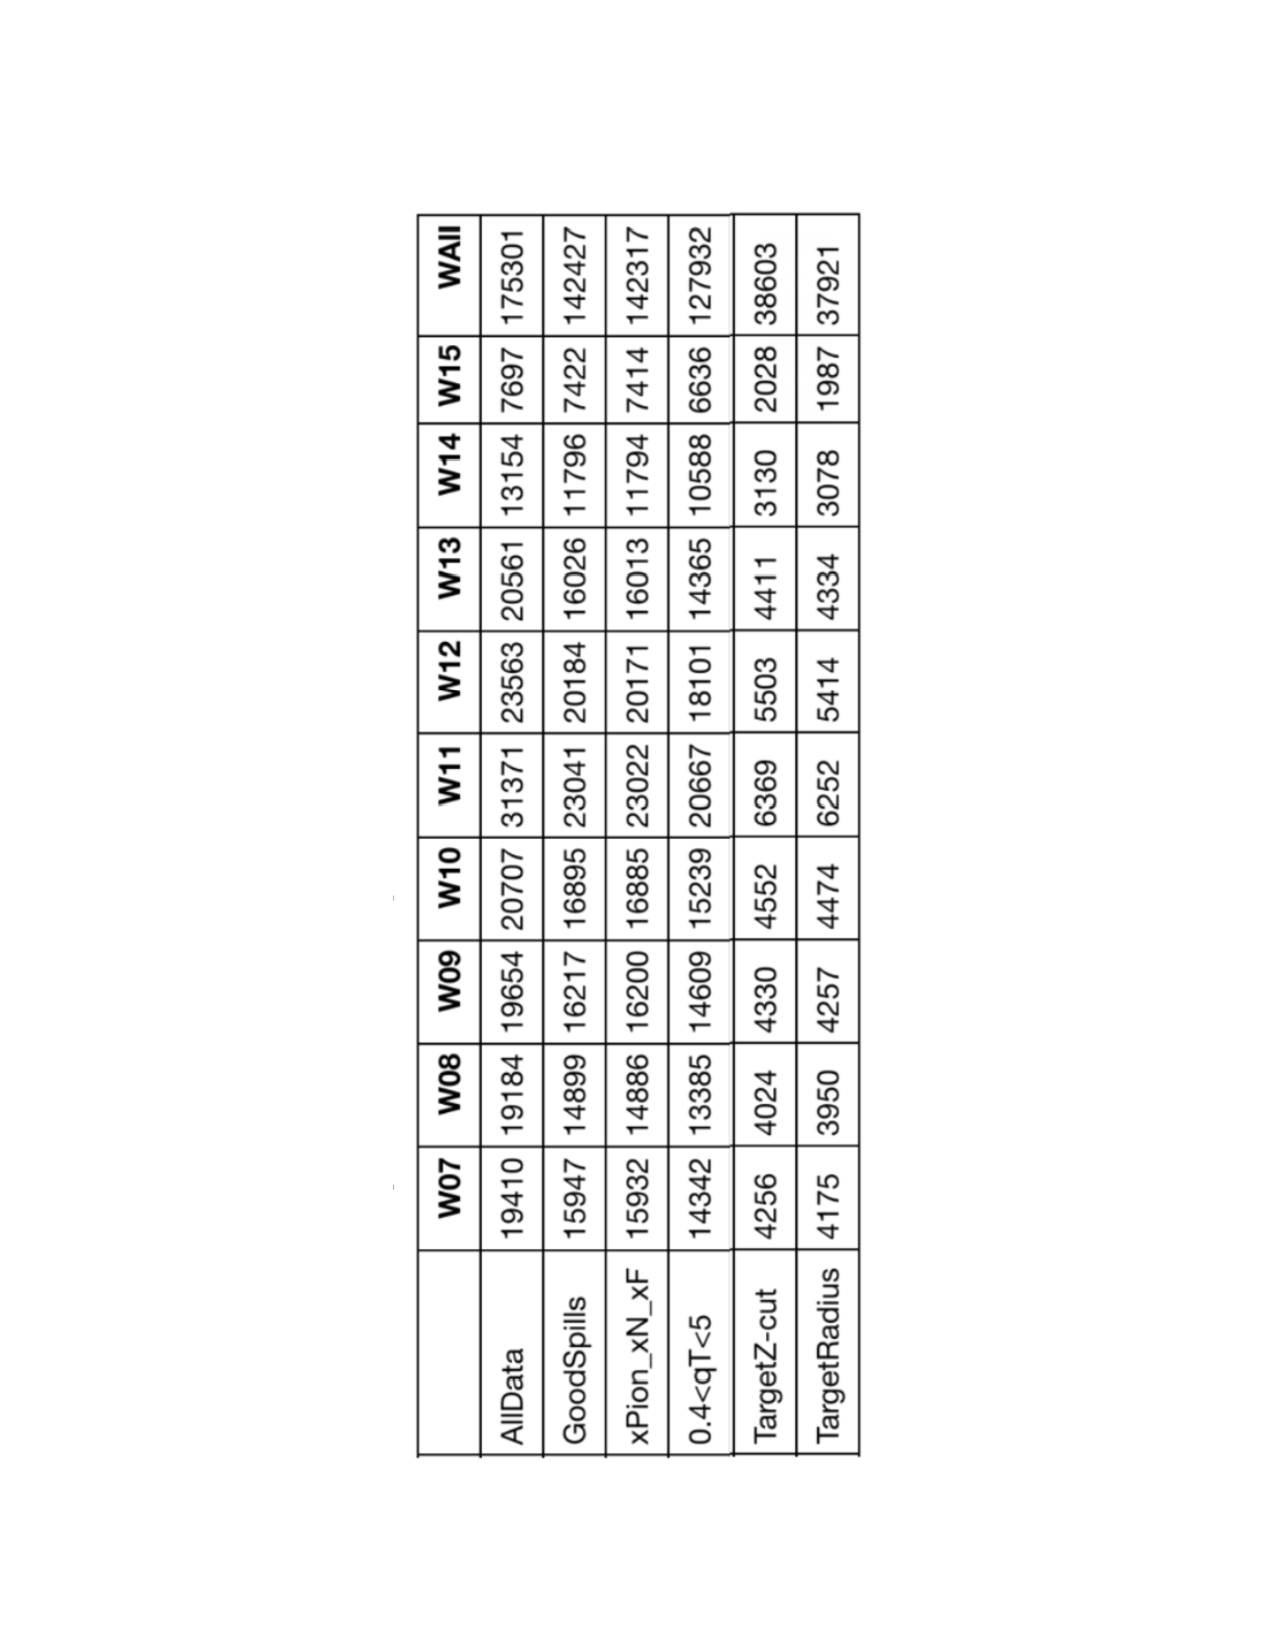
\includegraphics[width=\textwidth]{EventTable}
    \caption{Events}
    \label{fig::EventTable}%
  \end{center}
\end{figure}

\section{Extraction of Asymmetries} 

\subsection{Geometric Mean}
The number of physics counts, N, detected from any particular target with any
polarization can be written as
\begin{equation}
\mathrm{N} = \mathrm{L} * \sigma * \mathrm{a},
\end{equation}

\noindent
where L is the luminosity, $\sigma$ is the cross-section to produce such an
event and a is the acceptance.  In simple words, the number of counts detected
is the number of chances for an event to occur times the probability for an
event to occur and that the event will be detected.  To get spin-dependent
counts for the left, right asymmetry, the target, polarization and left or right
direction relative to the spin should be included in the counts formula.
Generically this can be written
\begin{equation}
  \label{eqn:indexedCount}
\mathrm{N}^{\uparrow(\downarrow)}_{\mathrm{target},\mathrm{Left(Right)}} =
\mathrm{a}^{\uparrow(\downarrow)}_{\mathrm{target},\mathrm{spectrometer \;
    direction}} * \mathrm{L}^{\uparrow(\downarrow)}_{\mathrm{target}} *
\sigma_{\mathrm{Left(Right)}},
\end{equation}

\noindent
where $^{\uparrow(\downarrow)}$ denotes the target polarization,
$_{\mathrm{target}}$ is either the upstream or downstream target
$_{\mathrm{Left(Right)}}$ is left or right of the spin direction and
${_\mathrm{spectrometer \; direction}}$ denotes which side of the spectrometer
the event was detected on.

The previous definitions of the detected counts all depend on the spectrometer
acceptance.  This is a problem because the spectrometer acceptance can change
with time and space and therefore can be dependent on the physical kinematics
which produced the event.  Such dependences can cause unphysical false
asymmetries in the measurement of A$_{\mathrm{N}}$ and must therefore be removed
or must included as systematic effects.

The geometric mean asymmetry method is a way to determine the left, right
asymmetry without acceptance effects from the spectrometer.  It is defined as
\begin{equation}
  \label{eqn:ANgeomean}
\frac{1}{\mathrm{P}}\frac{\sqrt{N_{\mathrm{target,
        Left}}^{\uparrow}N_{\mathrm{target, Left}}^{\downarrow}} -
  \sqrt{N_{\mathrm{target, Right}}^{\uparrow}N_{\mathrm{target,
        Right}}^{\downarrow}} }{\sqrt{N_{\mathrm{target,
        Left}}^{\uparrow}N_{\mathrm{target, Left}}^{\downarrow}} +
  \sqrt{N_{\mathrm{target, Right}}^{\uparrow}N_{\mathrm{target,
        Right}}^{\downarrow}} },
\end{equation}

\noindent
where P represents the fraction of polarized partons. Using
Eq. \ref{eqn:indexedCount} for the definition of counts, the geometric mean
asymmetry is
\begin{equation}
\frac{1}{\mathrm{P}}\frac{\kappa \sqrt{\sigma_{Left}\sigma_{Left}} -
  \sqrt{\sigma_{Right}\sigma_{Right}}}{\kappa \sqrt{\sigma_{Left}\sigma_{Left}}
  + \sqrt{\sigma_{Right}\sigma_{Right}}},
\end{equation}

\noindent
where $\kappa$ is a ratio of acceptances defined as
\begin{equation}
  \label{eqn:ANgeomean_expand}
\frac{\sqrt{\mathrm{a}^{\uparrow}_{\mathrm{target,Jura}}
    \mathrm{a}^{\downarrow}_{\mathrm{target,Saleve}}}}
     {\sqrt{\mathrm{a}^{\uparrow}_{\mathrm{target,Saleve}}
         \mathrm{a}^{\downarrow}_{\mathrm{target,Jura}}}}.
\end{equation}

\noindent
Here the detection side of spectrometer is specified by looking down the beam
line as either Jura to mean left or Saleve to mean right.  These relations of
Jura is left and Saleve is right are only strictly true if in the target frame
the polarization is pointing straight up or straight down.  In particular if the
beam particle and the target polarization do not make a right angle in the
laboratory frame this relation will no longer be strictly true but is an
approximation for ease of notation.

Relation \ref{eqn:ANgeomean_expand} is equal to A$_{\mathrm{N}}$ if $\kappa$ is
equal to one.  However time effects can vary $\kappa$ from unity. These effects
are estimated through false asymmetry analysis and included in the systematics.
Equation \ref{eqn:ANgeomean} is therefore to a good approximation an acceptance
free method to determine A$_{\mathrm{N}}$.  It is also defined for the upstream
and downstream targets independently and therefore can used as a consistency
check between the two targets.

\section{Systematic Studies}

\section{Results} 

% includi qui gli altri capitoli che aggiungerai. il nome del file da usare è quello del .tex Ti consiglio di mantere la struttura un capitolo = una cartella. Rende molto + semplcie la gestione dei file 
%\include{Chapter2/chapter2} 


\listoffigures

\listoftables


% ********************************** Back Matter *******************************
% Backmatter should be commented out, if you are using appendices after References
%\backmatter

% ********************************** Bibliography ******************************
\begin{spacing}{0.9}

% To use the conventional natbib style referencing
% Bibliography style previews: http://nodonn.tipido.net/bibstyle.php
% Reference styles: http://sites.stat.psu.edu/~surajit/present/bib.htm

%\bibliographystyle{apalike}
\bibliographystyle{unsrt}
 %\bibliographystyle{plainnat} % use this to have URLs listed in References
\cleardoublepage
\bibliography{References/references} % Path to your References.bib file


% If you would like to use BibLaTeX for your references, pass `custombib' as
% an option in the document class. The location of 'reference.bib' should be
% specified in the preamble.tex file in the custombib section.
% Comment out the lines related to natbib above and uncomment the following line.

%\printbibliography[heading=bibintoc, title={References}]


\end{spacing}

% ********************************** Appendices ********************************

%%\begin{appendices} % Using appendices environment for more functunality
%%
%%%\include{Appendix1/appendix1}
%%%\include{Appendix2/appendix2}
%%
%%\end{appendices}

% *************************************** Index ********************************
%\printthesisindex % If index is present

\end{document}
 
